\chapter{General machine learning methods}
In this master thesis, we will use several general machine learning methods in conjunction with each other. In this chapter we will introduce and explain these methods.

\section{Artificial Neural Networks (ANNs)}
In this section we will explain artificial neural networks (ANNs). In particular, we will focus on the multilayer perceptron (MLP). We refer to \cite[Chapter 11]{intro_to_ml_2014} and \cite{rong2016word2vec} when describing ANNs.

\begin{definition}
An artificial neuron (or unit) is a function which receives one or more inputs and a bias, and then sums them to produce an output, as illustrated in \cref{fig:artificial_neuron}; $\left\{ x_1, \ldots, x_K \right\}$ are the input values, $x_0$ is the bias, $\left\{ w_0, \ldots, w_K \right\}$ are the weights and $y$ is a scalar output. We denote $f$ as the activation function.
\end{definition}

\begin{figure}
    \centering
    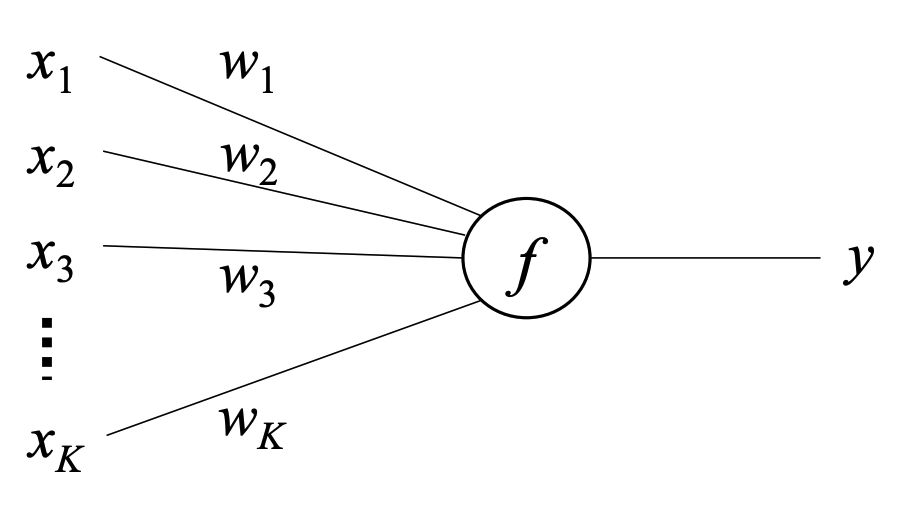
\includegraphics[width=8cm]{thesis/figures/artificial-neuron-rong-2014.png}
    \caption{An artificial neuron as illustrated by \cite[Figure 5]{rong2016word2vec}. Note that the bias is omitted from this illustration ($x_0=0$).}
    \label{fig:artificial_neuron}
\end{figure}

To produce the output of a single unit, we do the following
\begin{align}
    y = f(u)
\end{align}
where $u$ is the input of the neuron. $u$ is defined as
\begin{align}
    u = \sumlim{i=0}{K} w_i x_i
\end{align}
which is the weighted sum of the input values (including bias term) $\left\{ x_0, \ldots, x_K \right\}$ with $\left\{ w_0, \ldots, w_K \right\}$ as weights.

The bias term acts as a intercept value to make the model more general and is usually set to 1. For some models (e.g. word2vec, introduced in \cref{sec:word2vec-as-an-ann}), one does not include the bias term for the units in the neural network, i.e., we leave $x_0$ to be zero.

The choice of activation function $f$ is typically a non-linear function. Artificial neural networks use different activation functions such as ReLU, sigmoid or tanh to learn non-linear relationships in the data. We will come back to this in \cref{sec:activation-functions-ann}.

\newcommand{\layer}[2]{\left\{ {#1}_{#2} \right\}}

\begin{definition}
\label{def:layer_ann}
A layer $\layer{z}{j} = \left\{ z_1, z_2, \ldots, z_K \right\}$ of an artificial neural network is a collection of artificial neurons (unit). More formally, the layer $\layer{z}{j}$ can be described using an $N \times K$-dimensional weight matrix $W$, a $N$-dimensional bias vector $b$ and an activation function $f$; see \cref{eqn:artificial_layer}.
\end{definition}

\begin{align}
    \layer{z}{j} = f \left( W \cdot x + b \right)
    \label{eqn:artificial_layer}
\end{align}
where $x$ is a $K$-dimensional input vector. Note that we here separate $x$ and $b$ into separate vectors.

In the following subsections, we will go over the different types of layers in the ANN, namely the input, hidden and output layers.

\subsection{Input layer}
The first layer in the ANN is the input layer $\layer{x}{k} = \left\{ x_1, x_2, \ldots, x_K \right\}$. It is responsible for taking in input and passing it to the proceeding layer in the network. We illustrate the input layer in \cref{fig:input_layer_ann}.

\begin{figure}[H]
    \centering
    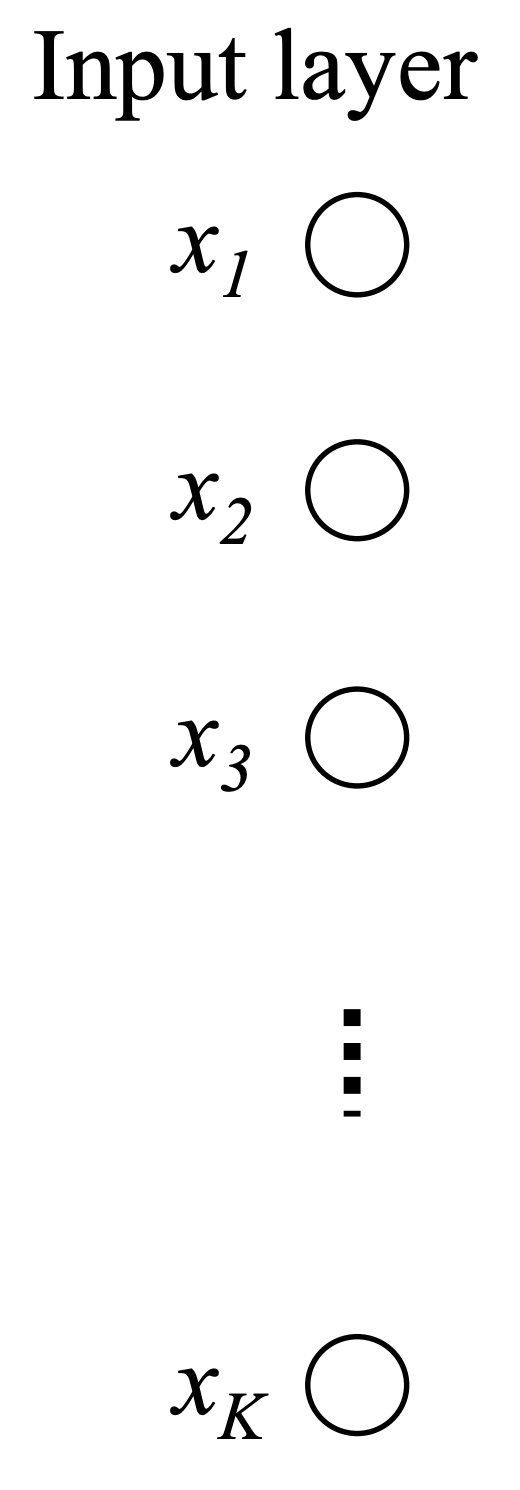
\includegraphics[height=7cm]{thesis/figures/ann-input-layer-rong-2014.png}
    \caption{Input layer in the ANN for a $K$-dimensional vector $x$. The bias $x_0$ is omitted from this figure. Illustration is taken from \cite[Figure 6]{rong2016word2vec}.}
    \label{fig:input_layer_ann}
\end{figure}

More formally, we define the input layer in \cref{eqn:input_layer_ann} using \cref{def:layer_ann}. The layer does not perform any changes to the incoming data and acts as a way for feeding data into the neural network. For this reason, \cref{eqn:input_layer_ann} uses the identity matrix $I_K$ as the weight matrix $W_{\layer{x}{k}}$, the $K$-dimensional bias vector $b_{\layer{x}{k}}$ consisting of all zeros and the identity function $id(x)=x$ as the activation function.
\begin{align}
    \label{eqn:input_layer_ann}
    \layer{x}{k}
    &= f_{\layer{x}{k}}(W_{\layer{x}{k}} \cdot x + b_{\layer{x}{k}}) \\
    &= id(I_K \cdot x) \\
    &= I_K \cdot x \\
    &= x
\end{align}
With this in mind, we look at the layer the input layer is connected to, namely the hidden layer.

\subsection{Hidden layer}
The hidden layer is the second layer in the ANN $\layer{h}{i} = \left\{ h_1, h_2, \ldots, h_N \right\}$, and is most commonly connected to the input layer. It should be noted, however, that we might have multiple hidden layers in the ANN (making the neural network deeper), connecting them to each other. For illustration purposes, we will assume that we only have one hidden layer in our neural network. The hidden layer is illustrated in \cref{fig:hidden_layer_ann}. Here we observe that every unit in the input layer is connected to the units in the hidden layer with a line. This is what we call fully connected layers, meaning that every unit is connected to each other.

\begin{figure}[H]
    \centering
    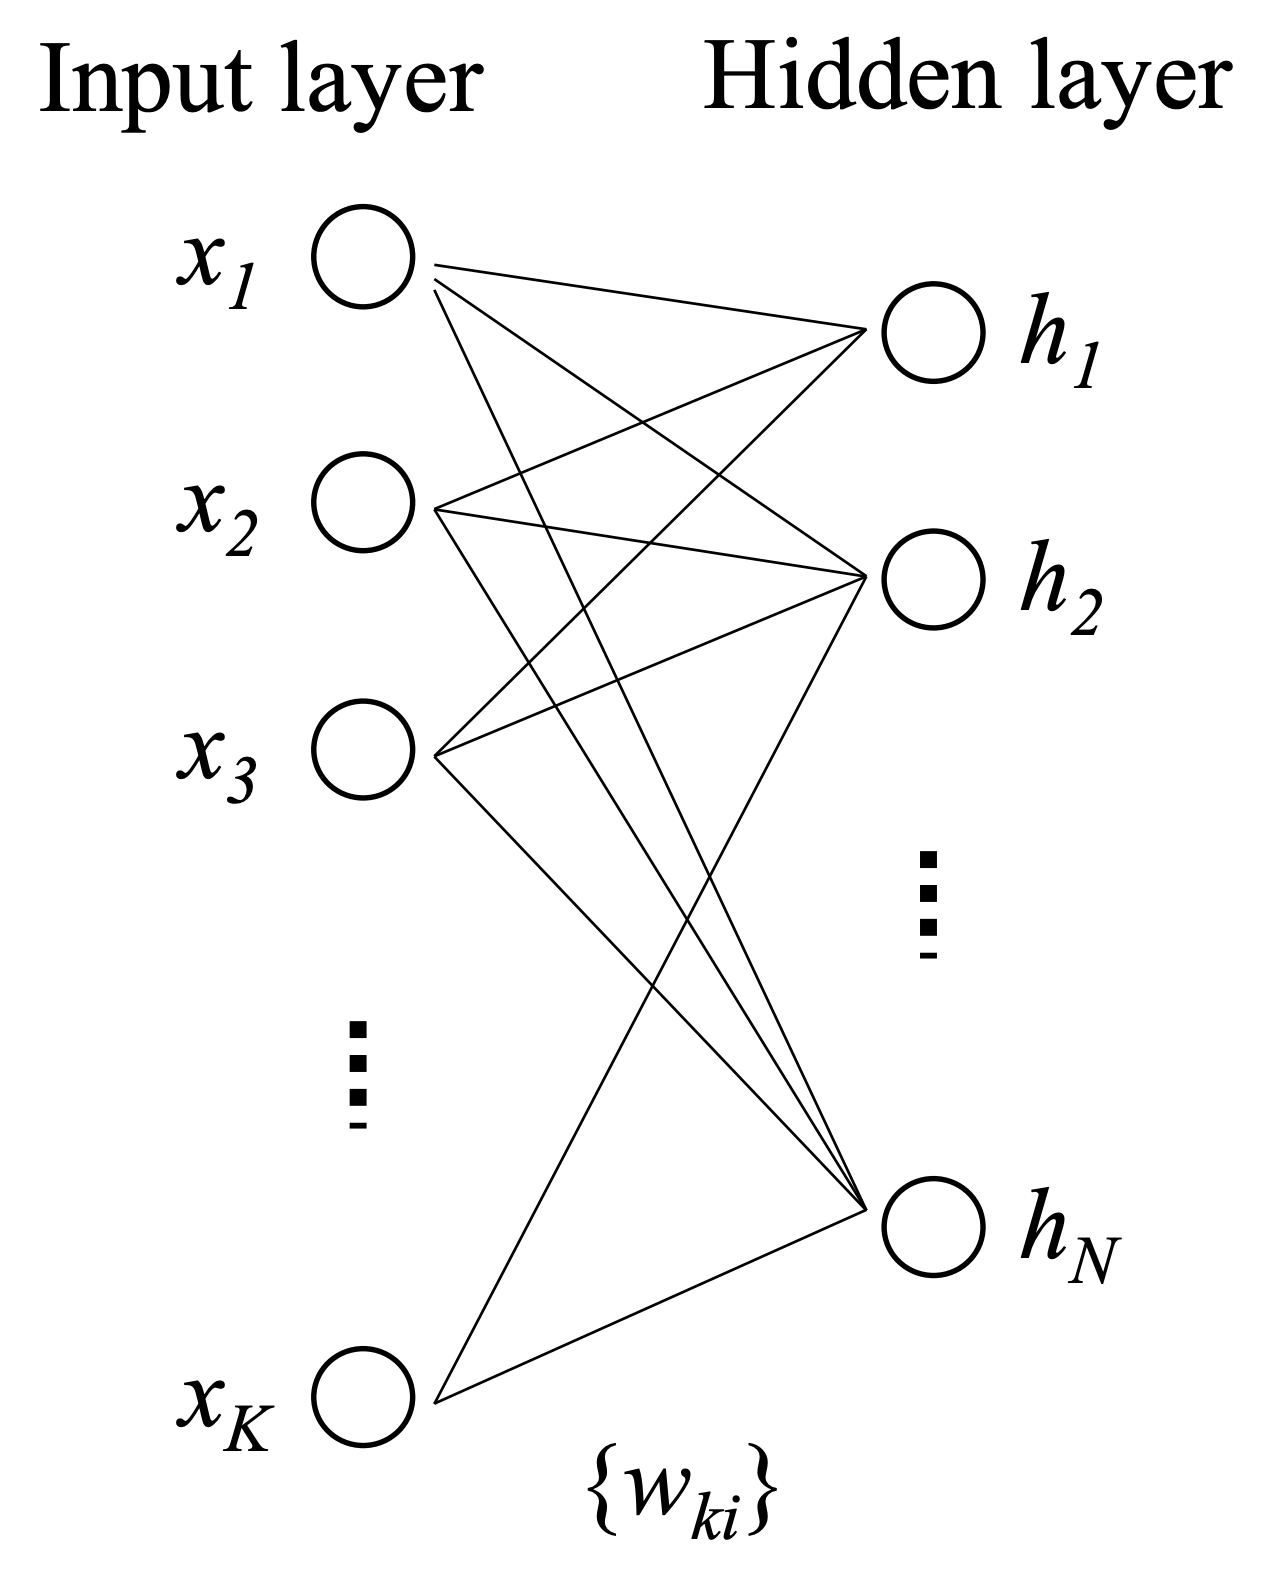
\includegraphics[height=7cm]{thesis/figures/ann-input-hidden-layer-rong-2014.png}
    \caption{Input to hidden layer in the ANN for a $K$-dimensional vector $x$, $N\times K$ dimensional weight matrix $\left\{ w_{ki} \right\}$ and a $N$-dimensional hidden layer $h$. Illustration is taken from \cite[Figure 6]{rong2016word2vec}.}
    \label{fig:hidden_layer_ann}
\end{figure}

We formalize the description of the hidden layer in \cref{eqn:hidden-layer-ann}
\begin{align}
    \label{eqn:hidden-layer-ann}
    \layer{h}{i} &= f_{\layer{h}{i}}(W_{\layer{h}{i}} \cdot \layer{x}{k} + b_{\layer{h}{i}})
\end{align}
where $f_{\layer{h}{i}}$ is a user-specified activation function, $W_{\layer{h}{i}}$ is an $N \times K$-dimensional weight matrix and $b_{\layer{h}{i}}$ is an $N$-dimensional bias vector.

The hidden layer tries to learn a latent representation of the input data $x$. We will explain how the neural network learns the latent representation when optimizers in \cref{sec:optimizers-ann}. Assuming that we have some $N$-dimensional latent representation of the data, we would like to connect it to the final layer in the neural network, namely the output layer.

\subsection{Output layer}
The last layer in the ANN is the output layer $\layer{y}{j} = \left\{ y_1, y_2, \ldots, y_M \right\}$ and is connected to the last hidden layer. Similar to the hidden layer, we connect each unit in the last hidden layer to each unit in the output layer, as illustrated in \cref{fig:mlp-one-hidden}.

\begin{figure}[H]
    \centering
    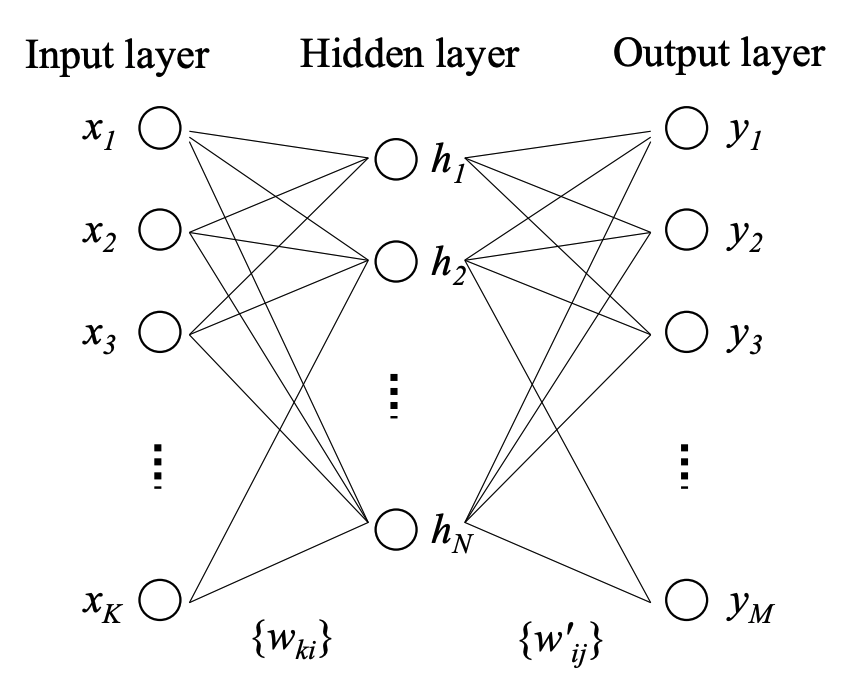
\includegraphics[width=8cm]{thesis/figures/multi-layer-neural-network-one-hidden-rong-2014.png}
    \caption{Multilayered perceptron (MLP) with one hidden layer, as illustrated by \cite[Figure 6]{rong2016word2vec}.}
    \label{fig:mlp-one-hidden}
\end{figure}

More formally, we define the output layer $\layer{y}{j}$ using a $M \times N$ weight matrix $W_{\layer{y}{j}}$, an $M$-dimensional bias vector $b_{\layer{y}{j}}$ and an activation function $f_{\layer{y}{j}}$, as seen in \cref{eqn:output-layer-ann}.

\begin{align}
    \label{eqn:output-layer-ann}
    \layer{y}{j} &= f_{\layer{y}{j}}(W_{\layer{y}{j}} \cdot \layer{h}{i} + b_{\layer{y}{j}})
\end{align}

We have now covered the different layers in an MLP, but have yet to cover the different choices of activation function $f$ in the neural network and how the MLP learns.

\subsection{Activation functions}
\label{sec:activation-functions-ann}
TODO
\begin{itemize}
    \item Simplest activation: identity function $id(x)=x$
    \item Sigmoid
    \item tanh
    \item ReLU
    \item Softmax
\end{itemize}

\subsection{Loss functions}
\label{sec:loss-functions-ann}
TODO
\begin{itemize}
    \item MSE
    \item Binary cross-entropy
    \item Categorical cross-entropy
\end{itemize}

\subsection{Optimizers}
\label{sec:optimizers-ann}
TODO
\begin{itemize}
    \item Gradient descent
    \item Stochastic gradient descent (SGD)
    \item Mini-batch gradient descent
    \item Mention other variants of gradient descent as well (Momentum, Adam, etc.)
\end{itemize}

\section{Clustering techniques}
TODO

\subsection{K-means clustering}
TODO

\subsection{Gaussian mixture models (GMMs)}
TODO

\subsection{Hierarchical clustering}
TODO

\subsection{Hierarchical Density-Based Spatial Clustering of Applications with Noise (HDBSCAN)}
TODO

\section{Dimensionality reduction techniques}
TODO

\subsection{Principal Component Analysis (PCA)}
TODO

\subsection{Uniform Manifold Approximation and Projection (UMAP)}
TODO

\subsection{t-distributed stochastic neighbor embedding (t-SNE)}
TODO